% ============================================================================
% kernscope: a unified C++ GPU-kernel tooling suite -- research report
% Compiled 2026-08-15.  All measurements are provenance-labeled and local to
% an AMD Radeon RX 7800 XT (gfx1101); no NVIDIA runtime numbers exist.
% Compile: pdflatex report.tex && bibtex report && pdflatex report.tex
%          && pdflatex report.tex
% ============================================================================
\documentclass[10pt]{article}

\usepackage[margin=1in]{geometry}
\usepackage[activate=false]{microtype}
\usepackage{amsmath,amssymb}
\usepackage[T1]{fontenc}
\usepackage[utf8]{inputenc}
\usepackage{graphicx}
\usepackage{booktabs}
\usepackage{tabularx}

\usepackage{xcolor}
\usepackage{caption}



\usepackage{tikz}
\usetikzlibrary{positioning,arrows.meta,shapes.geometric,calc}
\usepackage[round]{natbib}
\usepackage[colorlinks=true,linkcolor=blue!60!black,citecolor=green!40!black,urlcolor=blue!50!black]{hyperref}

\setlength{\parskip}{0.25em}
\setlength{\parindent}{1.2em}
\newcommand{\kst}[1]{\texttt{\detokenize{#1}}}
\newcommand{\tool}[1]{\texttt{\detokenize{#1}}}
\newcommand{\fpath}[1]{{\small\texttt{\detokenize{#1}}}}

\title{\vspace{-2.5em}\textbf{kernscope: A Unified C++ GPU-Kernel Tooling Suite}\\
\large Static Analysis, Autotuning, Verification, Capture/Replay, LLVM Passes, and Profiling in One Repository}
\author{Research Report}
\date{August 15, 2026}

\begin{document}
\sloppy\emergencystretch=3em

\maketitle

\begin{abstract}
\noindent
GPU kernel development today is fragmented across vendor profilers, simulators, ad-hoc
autotuners, and one-off static analyses that rarely share infrastructure or validate each
other's outputs. This report describes \textbf{kernscope}, a unified C++ GPU-kernel tooling
suite that integrates \emph{six} command-line tools --- a PTX/AMDGPU static analyzer, a
CUDA/HIP autotuning kernel generator, a static GPU kernel verifier, a kernel
capture-and-replay system, an out-of-tree LLVM-21 pass plugin, and a tiny CUDA/ROCm
profiler --- on top of one shared library stack (\kst{libs/}). The six tools form one
closed loop: a kernel enters as source or a running binary and leaves with
provenance-labeled, cross-validated evidence (profile $\rightarrow$ capture $\rightarrow$
analyze $\rightarrow$ transform/generate $\rightarrow$ verify $\rightarrow$ benchmark).
All engineering is grounded in the project's own research briefs, which survey GPUVerify,
PUG, ESBMC-GPU, Kerncap, HiRace, HGRD, Faial, IREE, Triton, FlashAttention, and the eBPF
verifier as prior art. Every measured number in this report was collected on a local AMD
Radeon RX 7800 XT (gfx1101) --- measured peaks of $591$\,GB/s DRAM read bandwidth,
$16.32$\,TFLOPS fp32, and $9.7$\,TB/s LDS --- under a strict honesty regime: reports carry
\kst{provenance.mode} = \emph{measured} $|$ \emph{projected}, NVIDIA runtime paths are
compile-only and owner-gated rentals, and \emph{no} NVIDIA runtime numbers are claimed.
\end{abstract}

\tableofcontents
\newpage

% ============================================================================
\section{Introduction}
% ============================================================================

\subsection{Motivation}

Writing high-performance GPU kernels is a multi-front activity. A developer must (a)
understand where time goes (profiling), (b) capture a failing or hot launch exactly as it
happens (record/replay), (c) understand the compiled ISA (static analysis), (d) generate
and select among launch-configuration variants (autotuning), (e) guarantee that a variant
does not introduce out-of-bounds accesses, races, or barrier divergence (verification),
and (f) rewrite the kernel at the IR level (compiler passes). In practice these tasks are
served by unrelated tools: \kst{nvprof}/\kst{Nsight Compute} or \kst{rocprofiler} for
profiling, CUPTI or rocprofiler-sdk samples for tracing, GPUVerify-class academic verifiers
for races, template-based autotuners, and bespoke LLVM passes. Each tool re-derives the
same architecture constants (register files, shared-memory sizes, occupancy limiters),
each uses a different report format, and none validates the others' outputs.

kernscope attacks this fragmentation with a single repository: six CLIs sharing a
library stack (\kst{libs/}), a common report engine with schema version and provenance,
and cross-tool edges that make the tools \emph{validate each other}. The profiler's
``memory-bound'' hint is cross-referenced against the static analyzer's findings on the
\emph{captured} kernel's ISA; the tuner gates variants through the verifier before
compiling them; the LLVM passes measure their before/after delta with the analyzer's
own metrics. This mirrors the loop that hardware-accelerator teams actually run, and it
is the report's central claim: that a unified toolchain produces evidence no single tool
could vouch for alone.

\subsection{Contributions}

\begin{itemize}
  \item \textbf{Six integrated CLIs} (\kst{tools/}): \kst{kernscope-analyze} (C1),
        \kst{kernscope-tune} (C2), \kst{kernscope-verify} (C3),
        \kst{kernscope-capture} (C4), \kst{kernscope-pass} (C5), and
        \kst{kernscope-profile} (C6).
  \item \textbf{A shared library stack} (\kst{libs/}): architecture DB with
        \emph{measured} gfx1101 peaks, PTX/AMDGPU parsers, occupancy and roofline
        engines, a correctness gate, a timing harness, a report engine, a CUPTI
        subscription layer, and a runtime wrapper with compile-only + mock backends.
  \item \textbf{A closed tool loop} wired end-to-end by \kst{scripts/demo.sh}, emitting one
        aggregated cross-tool report (\kst{reports/demo/report.json}).
  \item \textbf{A dual-path hardware strategy} that makes the suite fully testable with zero
        NVIDIA rentals: every NVIDIA capability has a compile-only implementation, while
        the HIP equivalents run live on the local gfx1101.
  \item \textbf{A four-layer test convention} and an honesty regime (provenance-labeled
        reports, owner-gated rentals) asserted by the CI gate.
  \item \textbf{Measured, provenance-labeled evidence}: this report quotes exact numbers
        from committed JSONL/JSON artifacts, never fabricated values.
\end{itemize}

\subsection{Reading guide}

Section~\ref{sec:background} positions each tool against prior art (the project's own
research briefs). Section~\ref{sec:arch} describes the system architecture with three
TikZ diagrams. Section~\ref{sec:tools} details the six tools with measured results.
Section~\ref{sec:methodology} states the dual-path hardware strategy, the four-layer test
convention, and the honesty guards. Section~\ref{sec:eval} summarizes the evaluation on
gfx1101. Sections~\ref{sec:limits}--\ref{sec:conclusion} discuss limitations, future
work, and conclusions. All measurements are quoted with their exact provenance path.

% ============================================================================
\section{Background and Related Work}
\label{sec:background}
% ============================================================================

The project grounds itself in a set of committed research briefs
(\fpath{docs/research/*.md}) --- one per tool plus \kst{owner-examples.md} and
\kst{rdna3-constants.md}. Each brief surveys prior art and cites primary sources; the
references in this report are drawn from those briefs and verified where noted in the
README.

\subsection{Roofline and the occupancy model (foundational)}

The performance-modeling foundation is the roofline model of \citet{roofline2009}, which
bound a kernel's attainable performance by the minimum of its compute ceiling and its
memory-bandwidth ceiling, with a ridge point at the arithmetic intensity (FLOPs/byte)
where the two cross. kernscope's \kst{libs/roofline} implements exactly this: given a
kernel family and a machine peak, it computes arithmetic intensity, ridge point, and
bound class. The occupancy model follows the CUDA C++ Programming Guide's definition of
occupancy as ``the ratio of the number of active warps to the maximum number of active
warps supported by the SM'' \citep{cudaProgrammingGuide}, with limiters computed from
device properties (registers, shared memory, threads, warps) exactly as
\kst{cudaOccupancyMaxActiveBlocksPerMultiprocessor} does. On the AMD side the guide's
constants are mirrored in \kst{rdna3-constants.md} and validated against LLVM's own
\kst{GCNSubtarget::computeOccupancy()} machinery. \citet{volkov2010} motivates
low-occupancy-but-high-ILP variants, which the tuner's shared-memory-limited configurations
exercise. Nsight Compute's \emph{Speed of Light} methodology \citep{nsightComputeSOL}
provides the diagnostic vocabulary the profiler adopts (compute-vs-memory percent of peak,
occupancy limiter, warp-stall reasoning).

\subsection{Static analysis of GPU assembly (C1)}

The analyzer brief surveys microbenchmark-driven architecture dissections: Volta
\citep{volta2018}, Turing \citep{turing2019}, Hopper \citep{hopper2024}, a
microbenchmark-driven analytical model across modern architectures \citep{model26}, and
CDNA3 shared-memory/latency exploration \citep{mall25}; the older
\citet{microbenchmark2010} dissected Fermi. Simulation frameworks (GPGPU-Sim
\citep{gpgpusim2009}, Accel-Sim \citep{accelsim2020}, MGPUSim, gem5) and binary
instrumentation (NVBit \citep{nvbit2019}) are referenced as alternatives that are far too
heavy for a quick static estimate. \citet{baremetal2017} grounds the register-limited
occupancy sweeps in measured microarchitecture behavior. The analyzer's core (register
pressure, occupancy + limiter, coalescing, bank conflicts, warp divergence, barrier
usage, tensor-core/MFMA/WMMA detection, spill detection) is a static re-implementation
of what these works measure dynamically.

\subsection{Autotuning and tensor-program compilation (C2)}

The tuner's prior art is the DSL/template generation line: Halide
\citep{halide2013} (algorithm/schedule separation and autoscheduling), TVM
\citep{tvm2018} and its answer to template-bound search, Ansor \citep{ansor2020},
and Triton \citep{triton2019} (tile-level IR with an autotuner over tile
parameters). The brief additionally cites the Halide autoscheduler variants
(\kst{mullapudi2016} analytic, \kst{li2018} RL, \kst{anderson2021} beam search)
and \citet{adamshalide2019} (tree-search scheduling). For attention workloads the
memory-bound claim follows FlashAttention \citep{flashattention2022} (``most operations in
Transformers are bottlenecked by memory accesses''), with decode-phase variants
following FlashDecoding++ \citep{flashdecoding2024}. Vendor tensor-core libraries
\citep{cublas,cudnn} and CUTLASS \citep{cutlass} define the bar the tuner's generated
matmul kernels are compared against; SCALE-Sim \citep{scalesim2019} represents the
simulator-based alternative. Kernel Tuner \citep{kerneltuner2024} is the closest
standalone autotuner prior art.

\subsection{GPU kernel verification (C3)}

The verifier brief is the richest. The methodological anchor is GPUVerify
\citep{gpuverify2012, gpuverify2015}: SDV semantics and the two-thread reduction that
reduces race/divergence checking to sequential program verification (with the CAV 2014
engineering retrospective \citep{gpuverify2014cav}). The line of symbolic execution begins
with PUG \citep{pug2010} (SMT-based verification of CUDA kernels), continues with SESA
\citep{sesa2014} and GKLEE \citep{gklee2012}. ESBMC-GPU \citep{esbmcgpu2017} contributes
context-bounded model checking including array bounds and pointer safety. Faial/FaialAA
\citep{faial2024} brings behavioral types over index expressions; its finding that of 191
DRF kernels \textbf{98\% need a specific thread-configuration assumption and 27\% need user
assertions} directly motivated kernscope-verify's launch-configuration ingestion
(Exact/UpperBound/Symbolic tiers). Recent work includes HiRace \citep{hirace2024}, HGRD
\citep{hgrd2026} (MLIR-level, dominance-based barrier intervals, host-parameter
constraints), and the dynamic race detectors GRace \citep{grace2011}, GMRace
\citep{gmrace2014}, CURD \citep{curd2018}, BARRACUDA \citep{barracuda2017}, ScoRD
\citep{scord2020}, and iGUARD \citep{iguard2021}. LLOV \citep{llov2020} demonstrates
static race freedom on LLVM IR; SPMD divergence abstraction \citep{spmddivergence2021}
underpins the barrier checks. The engineering template is the Linux eBPF verifier
\citep{ebpfVerifier}: a typed-register + bound-refinement engine with
\kst{check\_map\_access()}-style per-check probes, which kernscope-verify mirrors with
SCEV/LVI range machinery instead of tnums. SPIR-V validation \citep{spirvSpec} and
MemorySanitizer \citep{msan2015} (for the uninitialized-read class) complete the picture.

\subsection{Capture / replay (C4)}

The capture brief positions the work against Mneme \citep{mneme2023} (kernel record/replay
for tuning), the LLNL Record-Remix-Replay line \citep{r3-2026}, Kerncap
\citep{kerncap2026} (HSA-level extraction and isolation for HIP/Triton with
VA-faithful replay --- the closest complete system), Tally \citep{tally2024},
SIP \citep{sip2024}, KPerfIR \citep{kperfir2025}, and XSched (OSDI 2025, source of
\kst{cuda-intercept}). On the tooling side, CUPTI \citep{cupti}, PyTorch Kineto
\citep{kineto}, and rocprofiler-sdk \citep{rocprofilerSDK} define the two vendor
interception venues the suite uses. The project explicitly chose CUPTI
callback/injection over LD\_PRELOAD (research overturned the draft design) for NVIDIA,
and rocprofiler-sdk interception for the live HIP path.

\subsection{LLVM passes (C5)}

The memory-pass brief anchors on Triton \citep{triton2019}, IREE's MLIR GPU passes
\citep{iree} (GPUPromoteMatmulOperands, GPUReduceBankConflicts,
GPUConvertToCoalescedDMA), MLIR \citep{mlirCGO2021,mlirEndEra}, LLVM
\citep{llvm2004}, and the llvm-tutor \citep{llvmtutor} wiring model for out-of-tree
plugins. GVN's sparse predicated value numbering \citep{gargv2002} underpins the
redundant-load elimination pass.

\subsection{Profiling (C6)}

The profiler brief surveys CUPTI's activity API \citep{cupti}, Kineto's
correlation-id join and Chrome-trace output \citep{kineto}, NVBench's L2-flushed cold
timing, and Nsight Compute's sections/rules architecture \citep{nsightComputeSOL}; on the
ROCm side it documents rocprofiler-sdk's live interception and the rocprofiler/omniperf/
omnitrace ecosystem. The profiler re-implements the \emph{no-replay, launch-only} tier of
Nsight Compute (duration, grid/block, registers, smem, theoretical occupancy + limiter,
spill estimate) from Activity records alone, and degrades gracefully when counters are
unavailable.

% ============================================================================
\section{System Architecture}
\label{sec:arch}
% ============================================================================

\subsection{The closed tool loop}

The six tools are deliberately arranged as one loop, documented in
\kst{docs/architecture.md} and reproduced here:

\begin{figure}[ht]
  \centering
  \resizebox{\textwidth}{!}{% kernscope closed loop: profile -> capture -> analyze -> transform/generate -> verify -> benchmark
% Included from report.tex via \input.  Requires tikz + positioning + arrows.meta.
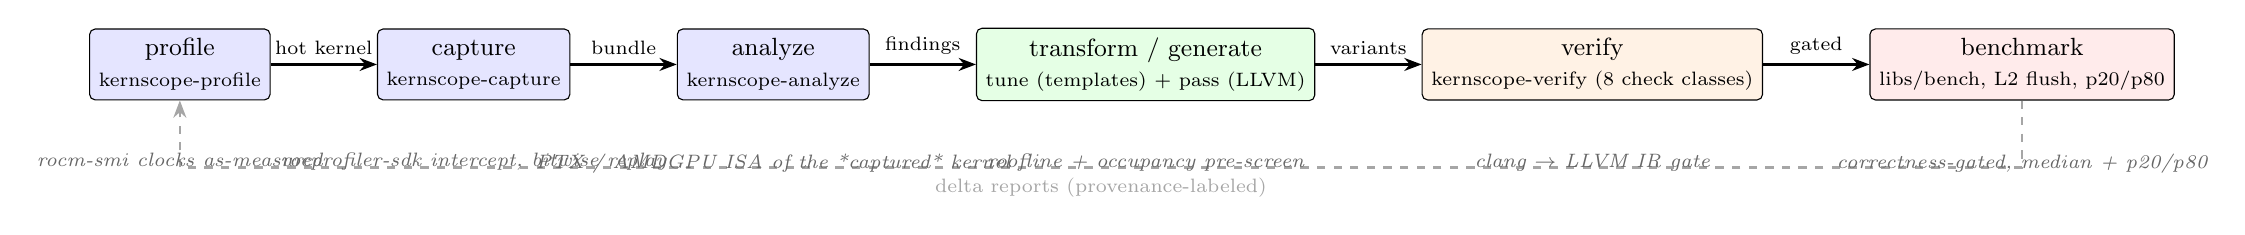
\begin{tikzpicture}[
    node distance=2.1cm and 1.35cm,
    box/.style={draw, rectangle, rounded corners=2pt, align=center,
                minimum height=9mm, minimum width=20mm, fill=#1,
                font=\small},
    box/.default=gray!12,
    lbl/.style={font=\scriptsize\itshape, text=black!60},
    arr/.style={-{Stealth[length=2.2mm]}, thick},
    feed/.style={-{Stealth[length=2.2mm]}, dashed, thick, gray!70},
  ]
  % ---- the six stages ----
  \node[box=blue!10]                 (prof)   {profile\\\scriptsize kernscope-profile};
  \node[box=blue!10, right=of prof]  (cap)    {capture\\\scriptsize kernscope-capture};
  \node[box=blue!10, right=of cap]   (ana)    {analyze\\\scriptsize kernscope-analyze};
  \node[box=green!10, right=of ana]  (trans)  {transform / generate\\\scriptsize tune (templates) + pass (LLVM)};
  \node[box=orange!10, right=of trans] (ver)  {verify\\\scriptsize kernscope-verify (8 check classes)};
  \node[box=red!8,    right=of ver]  (bench)  {benchmark\\\scriptsize libs/bench, L2 flush, p20/p80};

  % ---- main flow ----
  \draw[arr] (prof)  -- node[above, font=\scriptsize] {hot kernel}        (cap);
  \draw[arr] (cap)   -- node[above, font=\scriptsize] {bundle}            (ana);
  \draw[arr] (ana)   -- node[above, font=\scriptsize] {findings}          (trans);
  \draw[arr] (trans) -- node[above, font=\scriptsize] {variants}          (ver);
  \draw[arr] (ver)   -- node[above, font=\scriptsize] {gated}             (bench);

  % ---- closed-loop feedback ----
  \draw[feed] (bench.south) -- ++(0,-0.85) -| node[pos=0.25, below, font=\scriptsize]
             {delta reports (provenance-labeled)} (prof.south);

  % ---- tool annotations under the boxes ----
  \node[lbl, below=5.5mm of prof]   {rocm-smi clocks as-measured};
  \node[lbl, below=5.5mm of cap]    {rocprofiler-sdk intercept, bitwise replay};
  \node[lbl, below=5.5mm of ana]    {PTX / AMDGPU ISA of the *captured* kernel};
  \node[lbl, below=5.5mm of trans]  {roofline + occupancy pre-screen};
  \node[lbl, below=5.5mm of ver]    {clang $\to$ LLVM IR gate};
  \node[lbl, below=5.5mm of bench]  {correctness-gated, median + p20/p80};
\end{tikzpicture}
}
  \caption{The kernscope closed loop. A kernel enters at \emph{profile} (as a running
  binary) or at \emph{analyze} (as PTX/AMDGPU ISA) and exits from \emph{benchmark} with
  provenance-labeled delta reports that feed back into the loop.}
  \label{fig:loop}
\end{figure}

The loop is concrete, not decorative: \kst{scripts/demo.sh} runs all five observable
stages end-to-end under a 900\,s budget (it completes in 153\,s on the local machine,
\fpath{reports/demo/report.json}) and emits one aggregated report. The cross-tool edges
that close the loop are: \emph{profile $\rightarrow$ capture} (the profiler ranks hot
kernels; capture records the hot one), \emph{capture $\rightarrow$ analyze} (the analyzer
runs on the \emph{captured} kernel's disassembled ISA, not a hand-picked example),
\emph{capture $\rightarrow$ tune} (\kst{kernscope-tune --from-capture} searches launch
configurations over the captured bundle), \emph{tune $\rightarrow$ verify}
(\kst{kernscope-tune --verify} gates variants before compiling), \emph{pass
$\rightarrow$ analyze} (\kst{kernscope-pass-report --report-pipeline} measures
before/after deltas with analyzer metrics), and \emph{profile $\leftrightarrow$ analyze}
(profiler hints carry \kst{analyzer\_cross\_refs} to analyzer finding IDs).

\subsection{Library dependency graph}

All six tools link the shared stack; nothing depends downward on a tool
(\kst{docs/architecture.md}, asserted structurally by CMake):

\begin{figure}[ht]
  \centering
  \resizebox{\textwidth}{!}{% kernscope library dependency graph: libs/ -> tools/ (nothing depends downward on a tool)
% Included from report.tex via \input.  Requires tikz + positioning + arrows.meta.
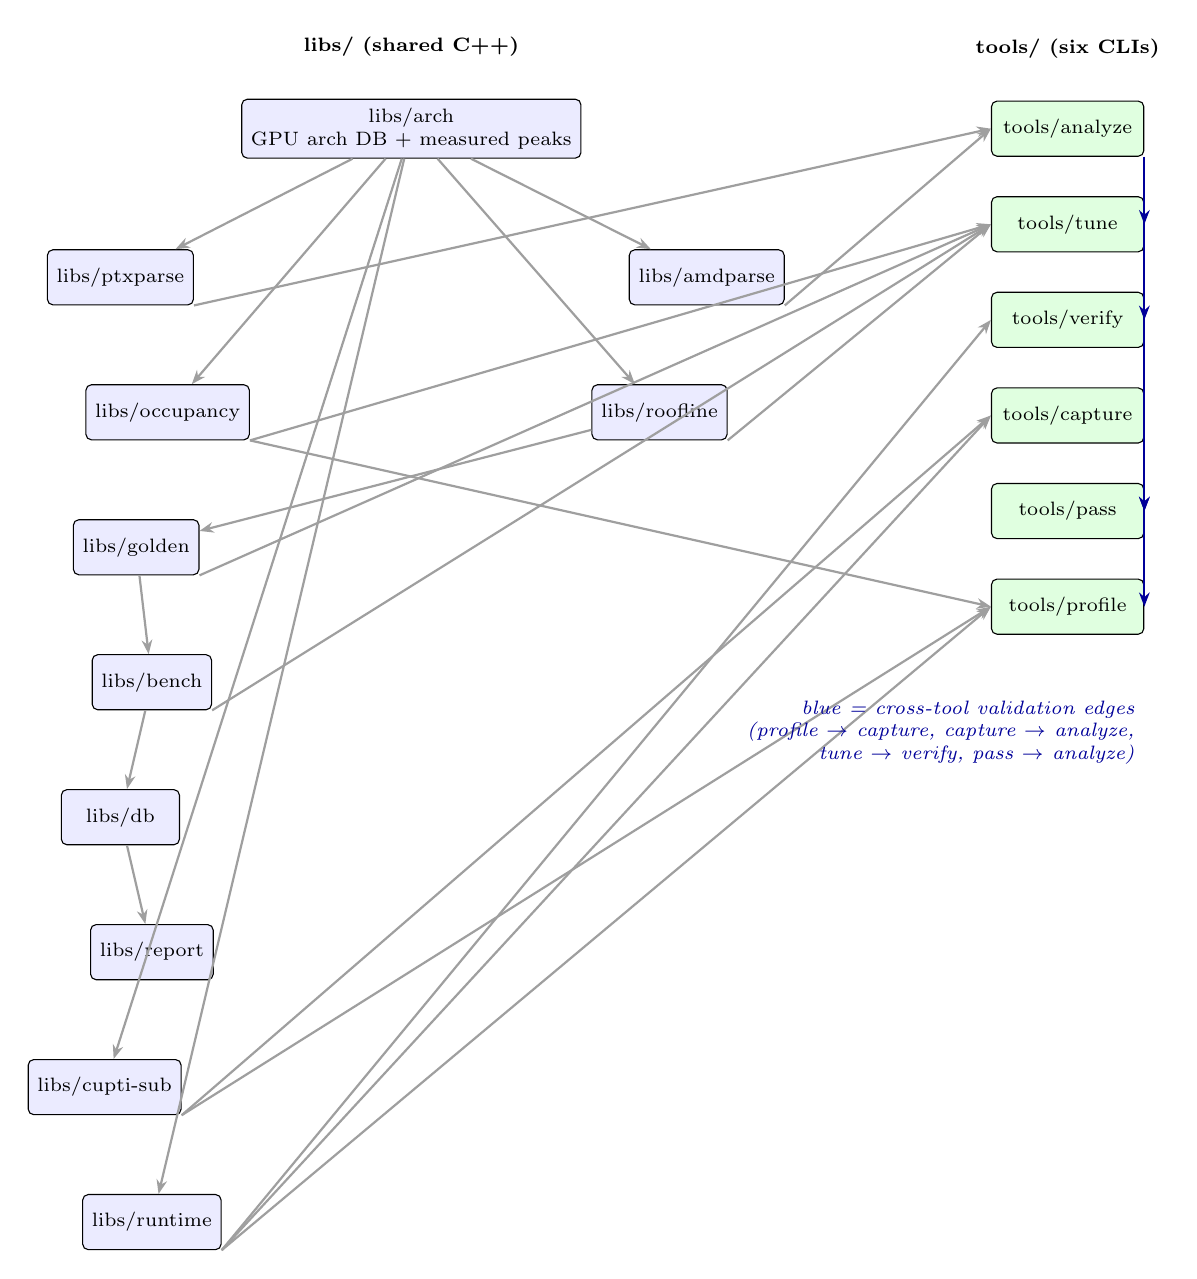
\begin{tikzpicture}[
    node distance=2.6cm and 0.5cm,
    lib/.style={draw, rectangle, rounded corners=2pt, align=center,
                minimum width=15mm, minimum height=7mm, fill=blue!8, font=\scriptsize},
    tool/.style={draw, rectangle, rounded corners=2pt, align=center,
                 minimum width=17mm, minimum height=7mm, fill=green!12, font=\scriptsize,
                 text width=17mm},
    edge/.style={-{Stealth[length=1.8mm]}, gray!75, thick},
    lbl/.style={font=\scriptsize\bfseries},
  ]
  % ---- libs tier ----
  \node[lib, minimum width=34mm] (arch) {libs/arch\\ \scriptsize GPU arch DB + measured peaks};
  \node[lib, below left=1.15cm and 0.6cm of arch]  (ptx)   {libs/ptxparse};
  \node[lib, below right=1.15cm and 0.6cm of arch] (amd)   {libs/amdparse};
  \node[lib, below=1.0cm of ptx, xshift=6mm]       (occ)   {libs/occupancy};
  \node[lib, below=1.0cm of amd, xshift=-6mm]      (rfl)   {libs/roofline};
  \node[lib, below=1.0cm of occ, xshift=-4mm]      (gold)  {libs/golden};
  \node[lib, below=1.0cm of gold, xshift=2mm]      (bench) {libs/bench};
  \node[lib, below=1.0cm of bench, xshift=-4mm]    (db)    {libs/db};
  \node[lib, below=1.0cm of db, xshift=4mm]        (rep)   {libs/report};
  \node[lib, below=1.0cm of rep, xshift=-6mm]      (cs)    {libs/cupti-sub};
  \node[lib, below=1.0cm of cs, xshift=6mm]        (rt)    {libs/runtime};

  % ---- tools tier (right column) ----
  \node[tool, right=5.2cm of arch, yshift=0cm] (t_ana)   {tools/analyze};
  \node[tool, below=0.5cm of t_ana]            (t_tune)  {tools/tune};
  \node[tool, below=0.5cm of t_tune]           (t_ver)   {tools/verify};
  \node[tool, below=0.5cm of t_ver]            (t_cap)   {tools/capture};
  \node[tool, below=0.5cm of t_cap]            (t_pass)  {tools/pass};
  \node[tool, below=0.5cm of t_pass]           (t_prof)  {tools/profile};

  % ---- lib -> lib edges (arch at the root) ----
  \draw[edge] (arch) -- (ptx);
  \draw[edge] (arch) -- (amd);
  \draw[edge] (arch) -- (occ);
  \draw[edge] (arch) -- (rfl);
  \draw[edge] (rfl)  -- (gold);
  \draw[edge] (gold) -- (bench);
  \draw[edge] (bench) -- (db);
  \draw[edge] (db)   -- (rep);
  \draw[edge] (arch) -- (cs);
  \draw[edge] (arch) -- (rt);

  % ---- lib -> tool edges ----
  \draw[edge] (ptx.south east)  -- (t_ana.west);
  \draw[edge] (amd.south east)  -- (t_ana.west);
  \draw[edge] (occ.south east)  -- (t_tune.west);
  \draw[edge] (rfl.south east)  -- (t_tune.west);
  \draw[edge] (gold.south east) -- (t_tune.west);
  \draw[edge] (bench.south east) -- (t_tune.west);
  \draw[edge] (rt.south east)   -- (t_ver.west);
  \draw[edge] (rt.south east)   -- (t_cap.west);
  \draw[edge] (cs.south east)   -- (t_cap.west);
  \draw[edge] (rt.south east)   -- (t_prof.west);
  \draw[edge] (cs.south east)   -- (t_prof.west);
  \draw[edge] (occ.south east)  -- (t_prof.west);

  % ---- tool-to-tool validation edges (the closed loop) ----
  \draw[edge, blue!60!black] (t_ana.south east) -- (t_tune.east);
  \draw[edge, blue!60!black] (t_ana.south east) -- (t_pass.east);
  \draw[edge, blue!60!black] (t_tune.east) -- (t_ver.east);
  \draw[edge, blue!60!black] (t_cap.south east) -- (t_prof.east);
  \draw[edge, blue!60!black] (t_ver.south east) -- (t_pass.east);

  \node[lbl, above=0.6cm of t_ana, anchor=base] {tools/ (six CLIs)};
  \node[lbl, above=0.6cm of arch, anchor=base]  {libs/ (shared C++)};
  \node[font=\scriptsize\itshape, text=blue!60!black, below=1.6cm of t_prof.east,
        anchor=east, align=right] {blue = cross-tool validation edges\\ (profile $\to$ capture, capture $\to$ analyze,\\ tune $\to$ verify, pass $\to$ analyze)};
\end{tikzpicture}
}
  \caption{Library dependency graph. \kst{libs/arch} (with its \emph{measured} gfx1101
  peaks) roots the stack; parsers feed the analyzer; occupancy/roofline/golden/bench/db
  feed the tuner; runtime + cupti-sub feed capture and profile. Blue edges are the
  cross-tool validation edges that close the loop of Figure~\ref{fig:loop}.}
  \label{fig:libgraph}
\end{figure}

Notable design decisions visible in the graph: \kst{libs/golden} is a correctness gate
(bf16 golden comparisons) rather than a timing helper; \kst{libs/bench} is a timing
harness with L2 flush and p20/p80 quantiles; \kst{libs/cupti-sub} is the single CUPTI
subscription, shared by capture and profile under a single-tool-scope contract;
\kst{libs/runtime} wraps cudart/hiprt with compile-only + mock backends so that
compile-gated NVIDIA paths run on AMD hardware; and \kst{tools/pass} shares the analyzer's
coalescing classification logic so before/after deltas use identical metrics.

\subsection{Dual-path hardware strategy}

Because the development machine has only an AMD RX 7800 XT (gfx1101), every NVIDIA
capability is given a second, live HIP implementation so the suite is testable with zero
rentals:

\begin{figure}[ht]
  \centering
  \resizebox{\textwidth}{!}{% kernscope dual-path hardware strategy: CUDA (compile-only, rental-gated) vs HIP (live on gfx1101)
% Included from report.tex via \input.  Requires tikz + positioning + arrows.meta.
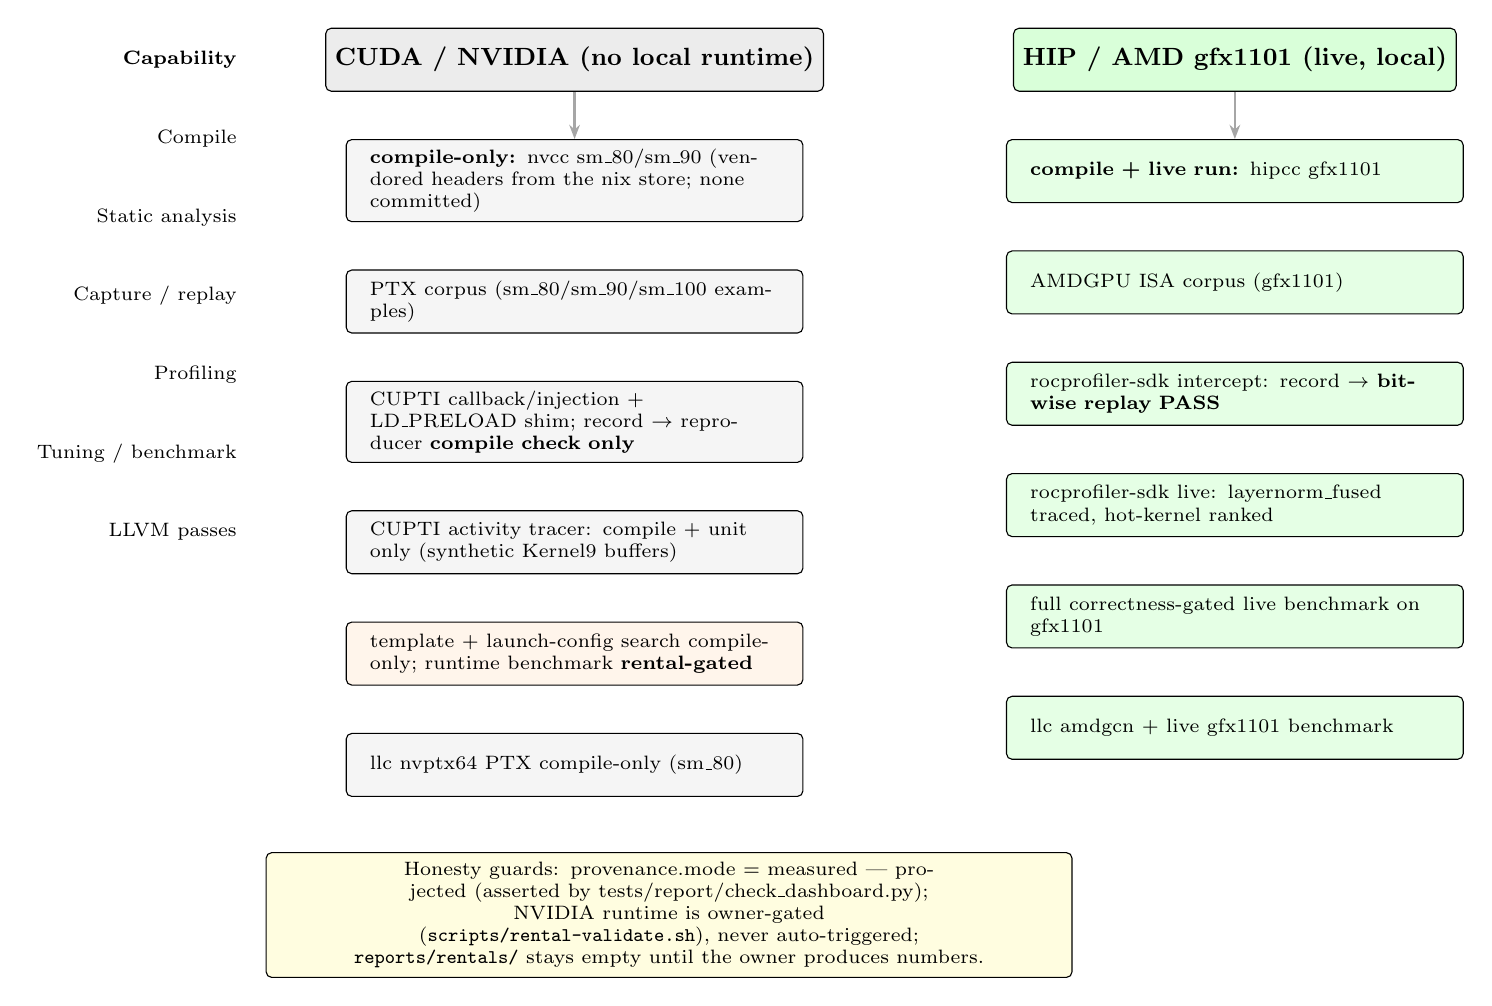
\begin{tikzpicture}[
    node distance=2.2cm and 0.5cm,
    head/.style={draw, rectangle, rounded corners=2pt, align=center,
                 minimum height=8mm, font=\small\bfseries},
    row/.style={draw, rectangle, rounded corners=2pt, align=left,
                minimum height=8mm, minimum width=58mm, font=\scriptsize,
                text width=52mm},
    live/.style={fill=green!10},
    compile/.style={fill=gray!8},
    gate/.style={fill=orange!8},
    arrow/.style={-{Stealth[length=1.8mm]}, thick, gray!70},
  ]
  % ---- column headers ----
  \node[head, fill=gray!15]  (h_cuda) {CUDA / NVIDIA (no local runtime)};
  \node[head, fill=green!15, right=2.4cm of h_cuda] (h_hip) {HIP / AMD gfx1101 (live, local)};

  % ---- capability rows (shared left label) ----
  \node[draw=none, left=1.0cm of h_cuda, anchor=east, font=\scriptsize\bfseries, align=right]
        (l0) {Capability};
  \node[draw=none, left=1.0cm of h_cuda, anchor=east, font=\scriptsize, align=right,
        yshift=-1.0cm] (l1) {Compile};
  \node[draw=none, left=1.0cm of h_cuda, anchor=east, font=\scriptsize, align=right,
        yshift=-2.0cm] (l2) {Static analysis};
  \node[draw=none, left=1.0cm of h_cuda, anchor=east, font=\scriptsize, align=right,
        yshift=-3.0cm] (l3) {Capture / replay};
  \node[draw=none, left=1.0cm of h_cuda, anchor=east, font=\scriptsize, align=right,
        yshift=-4.0cm] (l4) {Profiling};
  \node[draw=none, left=1.0cm of h_cuda, anchor=east, font=\scriptsize, align=right,
        yshift=-5.0cm] (l5) {Tuning / benchmark};
  \node[draw=none, left=1.0cm of h_cuda, anchor=east, font=\scriptsize, align=right,
        yshift=-6.0cm] (l6) {LLVM passes};

  % ---- CUDA column ----
  \node[row, compile, below=0.6cm of h_cuda]  (c1) {\textbf{compile-only:} nvcc sm\_80/sm\_90 (vendored headers from the nix store; none committed)};
  \node[row, compile, below=0.6cm of c1]      (c2) {PTX corpus (sm\_80/sm\_90/sm\_100 examples)};
  \node[row, compile, below=0.6cm of c2]      (c3) {CUPTI callback/injection + LD\_PRELOAD shim; record $\to$ reproducer \textbf{compile check only}};
  \node[row, compile, below=0.6cm of c3]      (c4) {CUPTI activity tracer: compile + unit only (synthetic Kernel9 buffers)};
  \node[row, gate,   below=0.6cm of c4]       (c5) {template + launch-config search compile-only; runtime benchmark \textbf{rental-gated}};
  \node[row, compile, below=0.6cm of c5]      (c6) {llc nvptx64 PTX compile-only (sm\_80)};

  % ---- HIP column ----
  \node[row, live, below=0.6cm of h_hip]  (h1) {\textbf{compile + live run:} hipcc gfx1101};
  \node[row, live, below=0.6cm of h1]     (h2) {AMDGPU ISA corpus (gfx1101)};
  \node[row, live, below=0.6cm of h2]     (h3) {rocprofiler-sdk intercept: record $\to$ \textbf{bitwise replay PASS}};
  \node[row, live, below=0.6cm of h3]     (h4) {rocprofiler-sdk live: layernorm\_fused traced, hot-kernel ranked};
  \node[row, live, below=0.6cm of h4]     (h5) {full correctness-gated live benchmark on gfx1101};
  \node[row, live, below=0.6cm of h5]     (h6) {llc amdgcn + live gfx1101 benchmark};

  % ---- headers row separator ----
  \draw[arrow] (h_cuda.south) -- (c1.north);
  \draw[arrow] (h_hip.south)  -- (h1.north);

  % ---- honesty banner ----
  \node[draw, rounded corners=2pt, fill=yellow!12, align=center, font=\scriptsize,
        below=0.7cm of c6, xshift=1.2cm, text width=100mm]
        {Honesty guards: provenance.mode = measured | projected (asserted by tests/report/check\_dashboard.py);\\
        NVIDIA runtime is owner-gated (\texttt{scripts/rental-validate.sh}), never auto-triggered;\\
        \texttt{reports/rentals/} stays empty until the owner produces numbers.};
\end{tikzpicture}
}
  \caption{Dual-path hardware strategy. CUDA/NVIDIA capabilities are compile-only or
  owner-gated rentals; HIP/AMD capabilities run live on gfx1101. The honesty banner
  (provenance.mode, \kst{reports/rentals/} emptiness, owner-gated
  \kst{scripts/rental-validate.sh}) is asserted by \kst{tests/report/check\_dashboard.py}.}
  \label{fig:dualpath}
\end{figure}

% ============================================================================
\section{The Six Tools}
\label{sec:tools}
% ============================================================================

This section describes each tool's design, implementation notes, and measured results.
All numbers are quoted exactly from the committed artifacts listed as provenance.

\subsection{C1 --- \kst{kernscope-analyze}: static analyzer}

\textbf{Design.} \kst{kernscope-analyze} consumes PTX (sm\_75--sm\_120) or AMDGPU ISA
(gfx90a/gfx942/gfx1101) and reports: register pressure, occupancy and its limiting
resource, coalescing class per access, shared-memory bank conflicts, warp divergence,
barrier usage, instruction mix, tensor-core/MFMA/WMMA usage, spill detection, and latency
bottlenecks. The occupancy engine re-implements the vendor formulas with the
\kst{libs/arch} constants (per-CC tables from the CUDA guide and \kst{rdna3-constants.md})
without depending on \texttt{cuda\_occupancy.h}.

\textbf{Measured results (golden kernel, projected).} On the committed
\kst{fused\_attention.ptx} fixture (PTX 8.5, sm\_86, 64-thread blocks = 2 warps, 67584 B
dynamic shared memory), the analyzer computes occupancy $0.375$, limiter
\texttt{registers}, $102$ registers/thread, 3 warnings and 3 suggestions
(\fpath{reports/dashboard.json} analyzer section; golden values in
\fpath{tests/fixtures/expected\_fused\_attention.json}). In the demo loop the analyzer ran
on the \emph{captured} layernorm ISA with 216 ALU ops and produced
\kst{possibly\_divergent\_branch} (warning) plus info findings
(\fpath{reports/demo/stage-3-analyze.json}).

\subsection{C2 --- \kst{kernscope-tune}: autotuning kernel generator}

\textbf{Design.} Template-based CUDA/HIP kernel generator (families: matmul, bias\_gelu,
softmax, layernorm, reduction, attention, elementwise). Each variant is
\emph{pre-screened} by occupancy + roofline (register/smem budget checks), \emph{gated} by
the bf16 golden correctness harness, \emph{timed} by \kst{libs/bench} (warmup, L2 flush,
median + p20/p80), and recorded in a JSON cache keyed by
\kst{(arch, family, shape-hash)}. The best variant is reported with its speedup over the
naive baseline (\kst{best.speedup >= 1.0} is asserted because the baseline is always
explored first).

\textbf{Measured results (gfx1101, live).} The committed matmul run
(\fpath{reports/tune/matmul-fnv1a64:e93d312338ce8fd7.jsonl} + \kst{.tunecache.json},
2026-08-15T14:36Z, \kst{provenance.mode=measured}) benchmarked 15 variants: the best
median is \textbf{0.4153\,ms} (tile\_k=32, 64$\times$64, 4 warps, 1 stage; occupancy 0.375,
limiter shared) and the worst is 3.106\,ms. The tunecache records 6 pre-screen rejections
--- e.g. \emph{``register budget exceeded: 512 acc fragment regs/thread (+32 overhead)
$>$ 256 max\_regs\_per\_thread on gfx1101''} and \emph{``smem budget exceeded: 66816 bytes
$>$ 65536 available''} --- and occupancy ranging 0.03125--0.875 across accepted configs.
An earlier-generation run is documented in the evidence ledger
(\fpath{.omo/evidence/task-29-gpu-kernel-suite.txt}): best 64$\times$64$\times$16, 4 warps,
1 stage at median \textbf{0.2027\,ms}, roofline position 1 (compute), occupancy 0.875,
\textbf{speedup 4.2$\times$} vs the naive baseline, 15 of 24 variants measured. The
currently committed \kst{reports/tune/} artifacts (a later run over a different search
space with pre-screening) show best 0.4153\,ms; the 0.2027\,ms figure is quoted from the
ledger, not the current JSONL, and the report treats them as two generations of the same
benchmark.

\subsection{C3 --- \kst{kernscope-verify}: static verifier}

\textbf{Design.} \kst{kernscope-verify} runs clang over CUDA/HIP source to LLVM IR and
applies 8 check classes: (1) out-of-bounds global/shared accesses, (2) shared-memory
bounds, (3) barriers (mismatch/divergence), (4) races, (5) illegal pointer arithmetic,
(6) divergent barriers, (7) uninitialized reads, (8) invalid address-space casts. Launch
configurations are ingested in three tiers (Exact / UpperBound / Symbolic); diagnostics
are eBPF-style with a per-function budget; verdicts gate tuner candidates
(\kst{kernscope-tune --verify}). It is a static IR-level verifier, not a formal prover;
the soundness scope (in-scope/out-of-scope classes, false-positive/negative classes) is
documented in \kst{docs/verify-soundness.md}.

\textbf{Measured results (projected corpus).} The committed manifest
(\fpath{tests/verify/manifest.json}, 34 entries across 19 corpus source files, 8 check
classes) yields verdicts: SAFE 18, MAY\_OOB 4, PTR\_OOB 4, MAY\_RACE 2, UNKNOWN\_RACE 1,
DIVERGENT\_BARRIER 1, BARRIER\_MISMATCH 1, INVALID\_ADDRSPACE\_CAST 1, MAY\_UNINIT\_READ 2
(\fpath{reports/dashboard.json} verify section, \kst{provenance.mode=projected}). The demo
stage-5 report shows the gate in action: one variant was \emph{verifier-gated} out before
compilation while 12 others compiled and benchmarked
(\fpath{reports/demo/stage-5-verify-tune.json}).

\subsection{C4 --- \kst{kernscope-capture}: capture and replay}

\textbf{Design.} On AMD, a rocprofiler-sdk intercept (LD\_PRELOAD shim) records kernel
dispatches with VA-faithful arguments and memory, then replays the bundle standalone with
bitwise-equal output validation. On NVIDIA, CUPTI callback/injection
(\kst{CUPTI\_API\_ENTER/EXIT}, \kst{CUDA\_INJECTION64\_PATH}) is primary, with an
LD\_PRELOAD fallback; the NVIDIA path is compile+unit tested locally and its live
behavior is owner-gated. The capture bundle format (v1) is schema-validated
(\fpath{docs/schema/capture-bundle.schema.json}).

\textbf{Measured results (gfx1101, live).} The demo captured the hot layernorm kernel
(\kst{\_Z15layernorm\_fusedPKtS0\_S0\_Ptfi.kd}, grid 1024$\times$1$\times$1, block
128$\times$1$\times$1) into \fpath{reports/demo/capture/bundle.v0} (3 blobs) and replayed it
with \textbf{bitwise PASS}: output SHA-256
\kst{a0027ed9a8ef2e3453aeb194aa64108c1f300a87fbfa292cca5222a725449eec} reproduced exactly
(\fpath{reports/demo/report.json} stage 2; \fpath{reports/dashboard.json} capture section,
\kst{replay\_bitwise\_equal=true}).

\subsection{C5 --- \kst{kernscope-pass}: LLVM passes}

\textbf{Design.} Out-of-tree LLVM-21 plugin (New Pass Manager,
\kst{PassPluginLibraryInfo}, loaded via \kst{-fpass-plugin} and \kst{-load-pass-plugin})
implementing: global-to-shared promotion, loop tiling, vectorized load/store rewrite,
shared-memory padding, redundant-load elimination, and a coalescing analysis pass. Tests
are lit/FileCheck; the before/after delta is measured by \kst{kernscope-pass-report
--report-pipeline} using the \emph{analyzer's own} metrics.

\textbf{Measured results (projected, compile-only).} On the layernorm kernel
(\fpath{reports/passes/layernorm/report.json} + \kst{llvm-diff.txt} +
\kst{coalesce\_before/after.txt}, pipeline
\kst{kernscope-tile,kernscope-promote,kernscope-vectorize,kernscope-pad,kernscope-coalesce}):
vector width $1 \rightarrow 4$, vectorized global loads $0 \rightarrow 12$
(\kst{pass\_reports.txt}: ``vectorized 48 loads, 0 stores (12 chains)''), widest access
$4\,\text{B} \rightarrow 16\,\text{B}$, and global-access count $64 \rightarrow 28$ with
uncoalesced $64 \rightarrow 16$ (delta $-48$; 12 partial accesses introduced). Register
estimate is unchanged at 175 (\fpath{reports/demo/stage-5-pass-delta.json}):
\kst{improved\_metrics} = [vectorized\_ld\_global, vector\_width, coalescing],
\kst{no\_transform=false}. gemm and softmax were correctly left \kst{no-transform}; all
three kernels compile to PTX with exit 0 after the pipeline
(\kst{ptx\_compile\_all\_exit0=true}). The tile pass declined on layernorm (``no canonical
\{0,+,1\} induction phi''). \fpath{reports/passes/bench/gfx1101-showcase-bench.jsonl}
holds the live gfx1101 benchmark of the transformed showcase.

\subsection{C6 --- \kst{kernscope-profile}: profiler}

\textbf{Design.} Kernel-launch tracing with per-kernel timing, occupancy/register/smem
estimates, hot-kernel ranking, and compiler-aware ``why slow'' diagnostics
(limiter decision tree over Activity-only inputs, per
\kst{docs/profile.md} and the profiler brief \S6). CUPTI on NVIDIA (compile + unit only);
rocprofiler-sdk live on AMD. The diagnostic vocabulary mirrors Nsight Compute's
launch-only tier \citep{nsightComputeSOL}.

\textbf{Measured results (gfx1101, live).} Tracing the \kst{layernorm\_fused} app
(\fpath{reports/demo/stage-1-profile.json}): 3 kernels, 19.6\,$\mu$s wall; the hot kernel
\kst{\_Z15layernorm\_fusedPKtS0\_S0\_Ptfi.kd} runs \textbf{9200\,ns (9.2\,$\mu$s)} with
\textbf{24 registers/thread}, occupancy 1 (limiter registers; diagnostic
\kst{limiter\_diag="memory"}), 1024 B shared, grid 1024$\times$1$\times$1, block
128$\times$1$\times$1. The profiler emits a \kst{memory\_bound} hint with evidence
arithmetic intensity 1.375, bytes-moved estimate 1048576, and ridge point 27.614
(computed from the measured $591\,$GB/s / $16.32\,$TF peaks). The same artifact records
the peak microbenchmarks (see Section~\ref{sec:eval}).

% ============================================================================
\section{Methodology}
\label{sec:methodology}
% ============================================================================

\subsection{Dual-path hardware strategy: CUDA compile-only + HIP live}

The suite pins a reproducible toolchain via devenv (LLVM/MLIR 21.1.8, CUDA 12.6
redistributables for sm\_80/sm\_90, ROCm 7.2.3; \kst{devenv.lock} committed and checked by
\kst{scripts/reproduce-all.sh}). Every NVIDIA-runtime capability has a compile-only
implementation that is fully exercised on the AMD machine, and a HIP implementation that
runs live on gfx1101 (Figure~\ref{fig:dualpath} in the architecture diagram,
Figure~\ref{fig:dualpath}). NVIDIA runtime validation is \emph{owner-gated}: only
\kst{scripts/rental-validate.sh} runs NVIDIA code, it is never auto-triggered, and its
output lands under \kst{reports/rentals/} only when the owner produces it (currently an
empty \kst{.gitkeep}).

\subsection{The four-layer test convention}

The CI gate (\kst{scripts/ci.sh}) enforces four layers:
\begin{enumerate}
  \item \textbf{gtest/ctest} -- the hardware-labeled suite
        (\kst{ctest -L "no-gpu|gpu-amd"}) with a non-decreasing count guard
        (\kst{scripts/ci-baseline.txt}, baseline $\ge 550$);
  \item \textbf{lit/FileCheck} -- the \kst{check-kernscope} lit suite for the pass
        plugin and verifier manifests;
  \item \textbf{NumPy bf16 golden harness} -- \kst{pytest tests/golden}, the reference
        bf16 golden comparisons that cross-check the C++ correctness gate;
  \item \textbf{generated-code compile checks} -- \kst{scripts/compile_checks.sh}:
        nvcc sm\_80/sm\_90 compile-only gates + hipcc gfx1101 compile gates + a live
        gfx1101 run with \kst{golden pass:true}.
\end{enumerate}
Committed fixtures are capped at 64\,MB total; NVIDIA headers are never vendored (the
nix store resolves \texttt{\#include <cuda\_occupancy.h>} at build time; ci.sh guards the
absence of vendored headers by filename and content).

\subsection{Honesty guards}

\begin{itemize}
  \item Every report carries \kst{schema\_version: "1.0"} and per-module
        \kst{provenance.mode} = \emph{measured} (live gfx1101) or \emph{projected}
        (static IR/PTX artifacts). \kst{tests/report/check\_dashboard.py} asserts the
        honesty flags; projected numbers are never presented as measured.
  \item The demo pass deltas are explicitly \kst{projected}: the
        \kst{reports/passes/*} artifacts are \kst{llc} compile-only outputs, and the
        report notes ``the measured numbers are the gfx1101 analog in the libs/db
        records (mode: measured)''.
  \item \kst{reports/rentals/} is empty; the dashboard machine note says
        ``LOCAL numbers only; rental numbers land under reports/rentals/ only when the
        owner produces them.''
  \item The gfx1101 peak numbers in \kst{libs/arch} are tagged
        \kst{peak\_source="measured-2026-08-14-gfx1101"} and are asserted (never
        datasheet numbers) by tests (\kst{arch\_test.cpp}, \kst{roofline\_test.cpp},
        \kst{bench\_live\_test.cpp}, \kst{check\_peaks.py}).
\end{itemize}

\subsection{Measured machine peaks (gfx1101, RX 7800 XT)}

\kst{kernscope-bench} (libs/bench, \kst{tool\_version kernscope-bench 0.1.0}) measured the
machine on 2026-08-14 and committed the raw records to
\fpath{reports/peaks/gfx1101-bench.jsonl} (device name, \kst{gcnArchName}, rocm-smi
sclk/mclk as-measured --- clocks were \emph{never} locked, no root). The derived peaks
reside in \kst{libs/arch} and \kst{libs/roofline}:

\begin{table}[ht]
  \centering
  \small
  \begin{tabularx}{\textwidth}{llrrX}
    \toprule
    Family & Rep & Median & Derived peak & Provenance \\
    \midrule
    \kst{peak\_flops} & FFMA loop & 13.51\,ms & \textbf{16.32 TF} &
      \fpath{gfx1101-bench.jsonl} rows 13/27/41 \\
    \kst{peak\_bw\_read} & 512\,MiB read & 0.907\,ms & \textbf{591 GB/s} &
      row 12/26/40; \kst{arch.h} 591.0\,GB/s \\
    \kst{peak\_bw\_d2d} & 1\,GiB D2D & 2.26--2.30\,ms & 467--475 GB/s &
      row 11/25/39; \kst{roofline.cpp} 476\,GB/s \\
    \kst{peak\_lds} & LDS R+W & 10.14--10.32\,ms & \textbf{9.7 TB/s} &
      row 14/28; \kst{arch.h} 9689.9\,GB/s \\
    \bottomrule
  \end{tabularx}
  \caption{Measured gfx1101 (AMD Radeon RX 7800 XT) machine peaks, 2026-08-14; every
  row is \texttt{provenance.mode=measured}. The fp32 figure is the register-resident FFMA peak
  ($\approx$15.6--16.4\,TF across runs); DRAM read peak $591\,$GB/s drives the roofline
  ridge point $27.61$ (ratio of the measured peaks
  $16.32\times10^{12}$\,FLOP/s and $591\times10^{9}$\,B/s).}
  \label{tab:peaks}
\end{table}

% ============================================================================
\section{Evaluation}
\label{sec:eval}
% ============================================================================

\noindent
\textbf{Hardware.} All live numbers are local gfx1101 (AMD Radeon RX 7800 XT, ROCm 7.2.3),
measured with as-is clocks. \textbf{There are no NVIDIA runtime numbers in this report or
in the repository}; PTX/cubin paths are compile-only, and NVIDIA runtime validation is
owner-gated via \kst{scripts/rental-validate.sh}.

\subsection{End-to-end loop (demo, 2026-08-15, gfx1101)}

\kst{scripts/demo.sh} runs the loop in 153\,s (budget 900\,s) and emits
\fpath{reports/demo/report.json}. Measured stages:
\begin{itemize}
  \item \textbf{profile} (stage 1): 3 kernels, hot kernel \kst{layernorm\_fused}
        9200\,ns, 24 regs/thread, occupancy 1, hint \kst{memory\_bound};
  \item \textbf{capture} (stage 2): bundle.v0 recorded, \textbf{bitwise replay PASS},
        output SHA-256 reproduced exactly;
  \item \textbf{analyze} (stage 3): analyzer on the \emph{captured} ISA, 216 ALU ops,
        \kst{possibly\_divergent\_branch} warning;
  \item \textbf{capture-tune} (stage 4): 4 candidates validated over the captured
        bundle; best block 256 at median \textbf{0.011880\,ms} (baseline block 128;
        speedup 1.0017$\times$; the report's own best-block figure is 0.012060\,ms,
        \fpath{reports/demo/stage-4-capture-tune.json});
  \item \textbf{verify-tune} (stage 5): \kst{verify\_gate=true}, 1 variant
        verifier-gated, 12 compiled; the bias\_gelu family's best
        (block 256, vec 4) runs median \textbf{0.17184\,ms} vs a 0.20332\,ms baseline
        (speedup 1.183$\times$), occupancy 1 (limiter registers), roofline position
        0.0845, memory bound at AI 2.33 (\fpath{reports/demo/stage-5-verify-tune.json}).
\end{itemize}
The cross-tool block of the report proves the loop is closed: the profiler's
\kst{memory\_bound} hint carries \kst{analyzer\_cross\_refs} pointing at analyzer
finding IDs derived from the captured ISA.

\subsection{Verifier corpus (projected)}

34 manifest entries, 19 source files, 8 check classes; verdict mix as reported in
Section~\ref{sec:tools} (C3), including the negative-path assurance that a
data-dependent index yields \kst{UNKNOWN\_RACE} (not SAFE/MAY\_RACE) and that a legal
generic-mediated pointer chain is not flagged (\kst{.omo/evidence/task-33/34}).

\subsection{Pass deltas (projected, compile-only)}

layernorm: vector width $1\rightarrow4$, vectorized global loads $0\rightarrow12$,
uncoalesced accesses $64\rightarrow16$ ($-48$), widest access $4\rightarrow16$\,B,
registers unchanged (175) --- \fpath{reports/passes/layernorm/*},
\fpath{reports/demo/stage-5-pass-delta.json}. gemm/softmax correctly
\kst{no-transform}. All before/after PTX compile cleanly (\kst{llc} exit 0).

\subsection{Tuning (measured, gfx1101)}

matmul: 15 variants measured, best median 0.4153\,ms (tile\_k=32, 64$\times$64, 4 warps,
1 stage, occupancy 0.375, limiter shared); worst 3.106\,ms; 6 pre-screen rejections
(register/smem budget); ledger-generation best 0.2027\,ms with speedup 4.2$\times$ and
occupancy 0.875 (\fpath{reports/tune/*}, \fpath{.omo/evidence/task-29}). flash\_attention:
24 compile-gated variants with occupancy 1.0 (limiter registers) for vec1/vec2 tiles and
shared-limited 0.25--0.75 for vec4.

\subsection{Analyzer goldens (projected)}

fused\_attention (sm\_86, PTX 8.5): occupancy 0.375, limiter \texttt{registers},
102 regs/thread, 67584 B dynamic shared, 3 warnings, 3 suggestions
(\fpath{reports/dashboard.json}, \fpath{tests/fixtures/expected\_fused\_attention.json}).

% ============================================================================
\section{Limitations}
\label{sec:limits}
% ============================================================================

\begin{itemize}
  \item \textbf{Single measured platform.} Every live number is gfx1101 (RX 7800 XT).
        Peaks were measured with as-is clocks (never locked, no root); the same kernel
        family on CDNA2/CDNA3 or any NVIDIA part is unverified.
  \item \textbf{No NVIDIA runtime evidence.} CUPTI capture/replay and CUPTI profiler
        tracing are compile+unit tested only; their live behavior on sm\_80/sm\_90 is
        unvalidated until the owner runs \kst{rental-validate.sh}. Reports never claim
        otherwise.
  \item \textbf{Projected pass deltas.} The \kst{reports/passes/*} before/after numbers
        are static IR/PTX artifacts (\kst{llc} compile-only); the measured gfx1101
        analog lives in the libs/db records and the showcase bench. Wall-clock
        speedups for the vectorized layernorm are therefore not claimed here.
  \item \textbf{Verifier soundness scope.} \kst{kernscope-verify} is a static IR-level
        verifier, not a formal prover: false-positive and false-negative classes exist
        and are documented in \kst{docs/verify-soundness.md} (e.g. SCEV-reconstruction
        failures degrade to \kst{UNKNOWN} verdicts at -O2).
  \item \textbf{Tuning search-space drift.} Two generations of the matmul benchmark
        (ledger 0.2027\,ms vs committed JSONL 0.4153\,ms) differ in search space and
        pre-screening; the report quotes both with provenance rather than averaging.
  \item \textbf{Benchmark noise.} Timing medians with p20/p80 are robust but the
        machine was shared with development activity; L2 flushing is applied but
        clock drift is not controlled.
\end{itemize}

% ============================================================================
\section{Future Work}
\label{sec:future}
% ============================================================================

\begin{itemize}
  \item \textbf{Owner-gated NVIDIA validation.} Run \kst{scripts/rental-validate.sh} on a
        rented A100/H100-class host; land results under \kst{reports/rentals/} with the
        same provenance schema, then extend the dashboard with an NVIDIA column.
  \item \textbf{CUDA 13 migration.} The versioned CUPTI record adapter
        (\kst{tools/profile/.../record\_adapter.h}, \kst{CUPTI\_API\_VERSION} 24) already
        pins the Kernel9$\rightarrow$Kernel10 surface so a header bump is a single-point
        compile error; exercise it against CUDA 13.
  \item \textbf{Verifier precision.} HGRD-style dominance-based barrier-interval
        splitting and host-parameter constraint propagation; PTX-level audit layer
        with spirv-val-style well-formedness gates \citep{hgrd2026,spirvSpec}.
  \item \textbf{Roofline-driven pass selection.} Wire the profiler's limiter diagnostics
        to pass selection (vectorize when memory-bound at AI below the ridge, as the
        layernorm case demonstrates) and to FlashAttention-style IO-aware tiling
        \citep{flashattention2022}.
  \item \textbf{LLM-generated kernel validation.} The verify gate + golden harness is
        a natural correctness harness for LLM-generated CUDA (cf.\ CUDAsmith's
        differential/EMI testing \citep{cudasmith2020}); a KernelBench-style workload
        sweep is a stated direction in the evidence ledger.
  \item \textbf{Multi-GPU occupancy.} Cluster-scoped shared memory (PTX AS 7) and
        Hopper/MI300X tile-level models \citep{hopper2024}.
\end{itemize}

% ============================================================================
\section{Conclusion}
\label{sec:conclusion}
% ============================================================================

kernscope demonstrates that a GPU-kernel tooling suite can be more than the sum of its
six CLIs: by sharing a library stack, a report schema, and --- critically --- the same
architectural constants and analysis metrics, the tools validate each other instead of
self-reporting. The closed loop (profile $\rightarrow$ capture $\rightarrow$ analyze
$\rightarrow$ transform/generate $\rightarrow$ verify $\rightarrow$ benchmark) is run
end-to-end in 153\,s on a local RX 7800 XT, with the profiler's memory-bound hint
cross-referenced against the analyzer's findings on the captured kernel's ISA and the
verifier gating every tuner candidate before compilation. The dual-path hardware
strategy delivers a suite that is fully testable with zero NVIDIA rentals while keeping
NVIDIA claims honest: every number is either measured on gfx1101 (591\,GB/s DRAM read,
16.32\,TFLOPS fp32, 9.7\,TB/s LDS, 0.4153\,ms best matmul variant, bitwise-equal capture
replay) or explicitly projected from compile-only artifacts. The repository's committed
research briefs ground every design decision in prior art from GPUVerify to Kerncap, and
this report inherits that grounding. The result is a reproducible, honest, and
cross-validated evidence base for GPU kernel optimization --- and a template for how
toolchains for one domain should be built.

\bibliographystyle{plainnat}
\bibliography{report}

\end{document}
